% vim: set spell spelllang=es syntax=tex :

\section{Fútbol de robots}

La \emph{RoboCup} (abreviación del ingles \emph{Robot World Cup}) es una
competencia internacional celebrada desde 1997, donde equipos de robots juegan
una versión simplificada del fútbol. Su finalidad es la de poner a prueba los
avances en distintas áreas de conocimiento como la inteligencia artificial,
visión por computadora y robótica. Existen cinco ligas distintas que van desde
el ambiente y robots simulados a robots humanoides con visión local. De estas,
la mas antigua es la liga de tamaño pequeño (\emph{SSL}, del ingles \emph{Small
Size League}).

Un partido de la \emph{SSL} enfrenta a dos equipos de seis robots, que deben
tener un tamaño menor que un cilindro de 9$cm$ de radio y 15$cm$ de
alto\cite{sslrules2015}. Los robots tienen capacidad de procesamiento reducida,
delegando la toma de decisiones a la computadora de su equipo. Estas a su vez
perciben el ambiente a través de un sistema de visión global centralizado
compartido. Este sistema de visión consta de un conjunto de cámaras montadas
sobre distintas áreas del campo de juego conectadas a una computadora donde se
ejecuta el sistema de visión. El sistema detecta la posición y orientación de
cada uno de los robots y la posición de la pelota, y reporta esta información a
las computadoras que controlan los equipos. En la figura \ref{sistemaVG} se
presenta un diagrama mostrando esta estructura.

\begin{figure}[!h]

	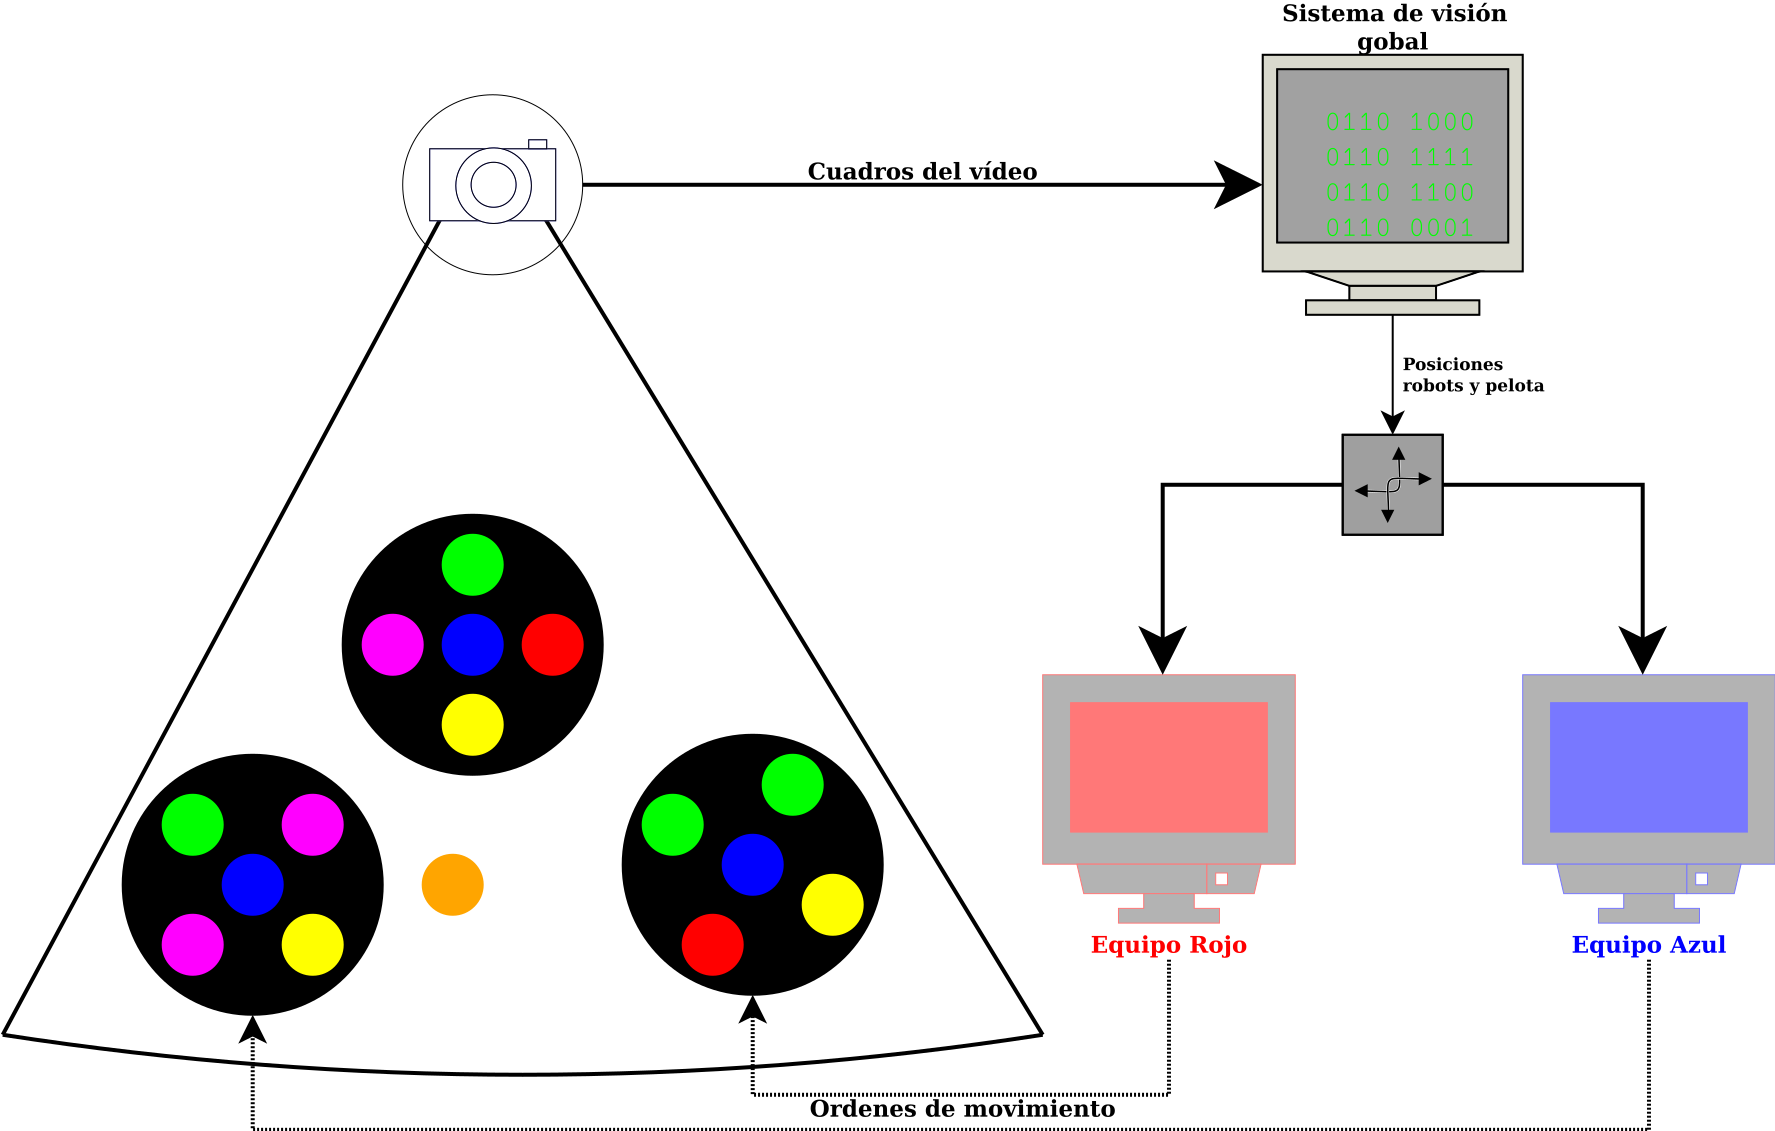
\includegraphics[width=\textwidth]{img/sistemaVG.pdf}
	\caption{Estructura de comunicación del sistema de visión global en
	fútbol de robots de la \emph{SSL}.}
	\label{sistemaVG}

\end{figure}

El uso de este sistema centralizado permite a los participantes abstraerse de
los problemas de la visión por computadora y enfocarse en la estrategia del
juego. Además, permite que las tareas de calibración y montaje de las cámaras se
realicen una sola vez para cada campo de juego en vez de para cada partido.

Originalmente el tamaño de la cancha era de 4,9$m$x3,4$m$, lo que permitía que
todo el campo de juego fuera observado con una sola cámara. Luego se opto por
dos tipos de canchas en los partidos de la \emph{SSL}: las canchas de tamaño
simple, con un tamaño de 6,05$m$x4,05$m$ para las cuales se utilizan dos
cámaras, una sobre cada media cancha, y las de tamaño doble, con un tamaño de
8,09$m$x6,05$m$, que utilizan cuatro cámaras, una por cada mitad de cada media
cancha. Desde el 2015 las canchas de tamaño doble son las utilizadas de forma
predeterminada\cite{sslrules2015}. Con este cambio se espera permitir la
exploración de nuevas tácticas por parte de los equipos, ya que mayor área
permite mayor movilidad. Sin embargo, esto trae aparejado el problema de que en
las canchas de tamaño doble se debe procesar cuatro veces la información que en
las canchas originales.

Aunque las reglas de la \emph{SSL} no establecen una resolución o taza de
cuadros para los vídeos capturados por las cámaras, en \cite{torres2014} se
comprobó que para una cancha de tamaño simple, con un vídeo con una resolución
de 352x288 píxeles, es suficiente para encontrar los robots y pelota en el
$99\%$ de los cuadros. Por lo tanto, un vídeo de 800x600 píxeles es suficiente
para la totalidad de una cancha de tamaño doble.
